\documentclass[b5paper,11pt]{book}

\usepackage{geometry} 					% поля страницы

\usepackage{cmap}                       % Поддержка поиска русских слов в PDF (pdflatex)
\usepackage[T2A]{fontenc}				% Поддержка русских букв
\usepackage[utf8]{inputenc}            	% Выбор языка и кодировки
\usepackage[english, russian]{babel}	% Языки: русский, английский

\usepackage[unicode]{hyperref}			% Русский язык для оглавления pdf
\usepackage{bookmark}					% Оглавление в pdf
\usepackage{graphicx} 					% Подключаем пакет работы с графикой

\usepackage{amsmath,amssymb}

\graphicspath{{../../images/}} 			% Пути к изображениям

\geometry{left=2cm,right=2cm,top=2cm,bottom=2cm}	% Геомтерия страницы

\usepackage[
%	autolang=hyphen,
language=auto,
autolang=other,
backend=biber,
style=gost-numeric
]{biblatex}
\addbibresource{tbi.bib}

\DeclareSourcemap{
	\maps[datatype=bibtex, overwrite]{
		\map{
			\step[fieldset=langid, fieldvalue=english]
			\step[fieldset=doi, null]
			\step[fieldset=issn, null]
			\step[fieldset=isbn, null]
			\step[fieldset=url, null]
			\step[fieldsource=language, fieldset=langid, origfieldval]
		}
	}
}

\let\cleardoublepage\clearpage

\begin{document}
	\begin{titlepage}
		\begin{center}
			{\bfseries  Федеральное государственное автономное \\
				образовательное учреждение высшего образования\\
				<<Российский университет дружбы народов>>
				
			}

			\vspace{-5pt}
			\noindent\rule{\textwidth}{2pt}
			
			\vspace{50pt}
			{\Large\bfseries А.\,И.~Панов}
			
			\vspace{100pt}
			{\Huge\bfseries Теоретические основы информатики}
			
			\vspace{20pt}
			{\Large\itshape Учебно-методическое пособие}
			
			\vfill
			{\bfseries Москва\\
				Российский университет дружбы народов\\
				2015
			}
		\end{center}
	\end{titlepage}
	
	\chapter*{}
	
	В пособии рассмотрены основные понятия теоретических основ информатики. Информатика (или, как принято называть ее за рубежом, компьютерные науки или Сomputer Science) в настоящее время представляет из себя набор большого количества дисциплин, которые не смотря на свою разнородность как по применяемым методам и подходам, так и по методологии исследований, обладают тем не менее общими теоретическими основами. Центральной идеей в представленном курсе является рассмотрение вопросов, связанных с обработкой, хранением, передачей и приобретением информации с точки зрения знаковых систем. Данная идея позволяет ввести многие методы и задачи, возникающие и в теории измерения количества информации, и в теории кодирования, и в теории программирования, с единых позиций и построить общую картину теоретических основ компьютерных наук.
	
	Особое внимание уделено рассмотрению основ такой области информатики и кибернетики как искусственный интеллект, что, по мнению автора, обусловлено текущими запросами общества на всеобщую интеллектуализацию операций и более понятные и близкие человеку машинные интерфейсы. 
	
	Пособие не требует от читателя глубоких познаний в области информатики и искусственного интеллекта и предназначено для будущих специалистов в области компьютерных наук (Computer Science).
	
	
	\tableofcontents %% содержание
		
	\chapter*{Введение}
	\addcontentsline{toc}{chapter}{Введение}
	Теоретические основы информатики "--- это область информатики (компьютерных наук, Computer Science), которая рассматривает теоретические вопросы, связанные с получением, обработкой, хранением, передачей и преобразованием информации. Многие задачи, рассматриваемые в этой области опираются на определения и методы таких разделов математики, как теория вероятности и математическая статистика. Все попытки дать общие определения информатики и информации сталкиваются с проблемой замкнутого цикла, который отличным литературным языком описан Станиславом Лемом \cite{Lem2015}. В этой связи во многих курсах теоретических основ информатики предпринимается попытка построения общего представления об информации с помощью конкретных примеров ее измерения, получения, обработки и т.~п., т.~е. дается эксплицитное определение на примерах использования. 
	
	В данном пособии используется иной подход, связанные с рассмотрением вопросов связанных с использованием в качестве носителя информации \textit{знаковых систем}. Таким образом, вместо определения информации мы будем вводить понятия системы и знака, с помощью которых будут определены и основные операции с информацией, сводящиеся к операциям со знаковыми системами.
	
	\begin{figure}[h]
		\centering
		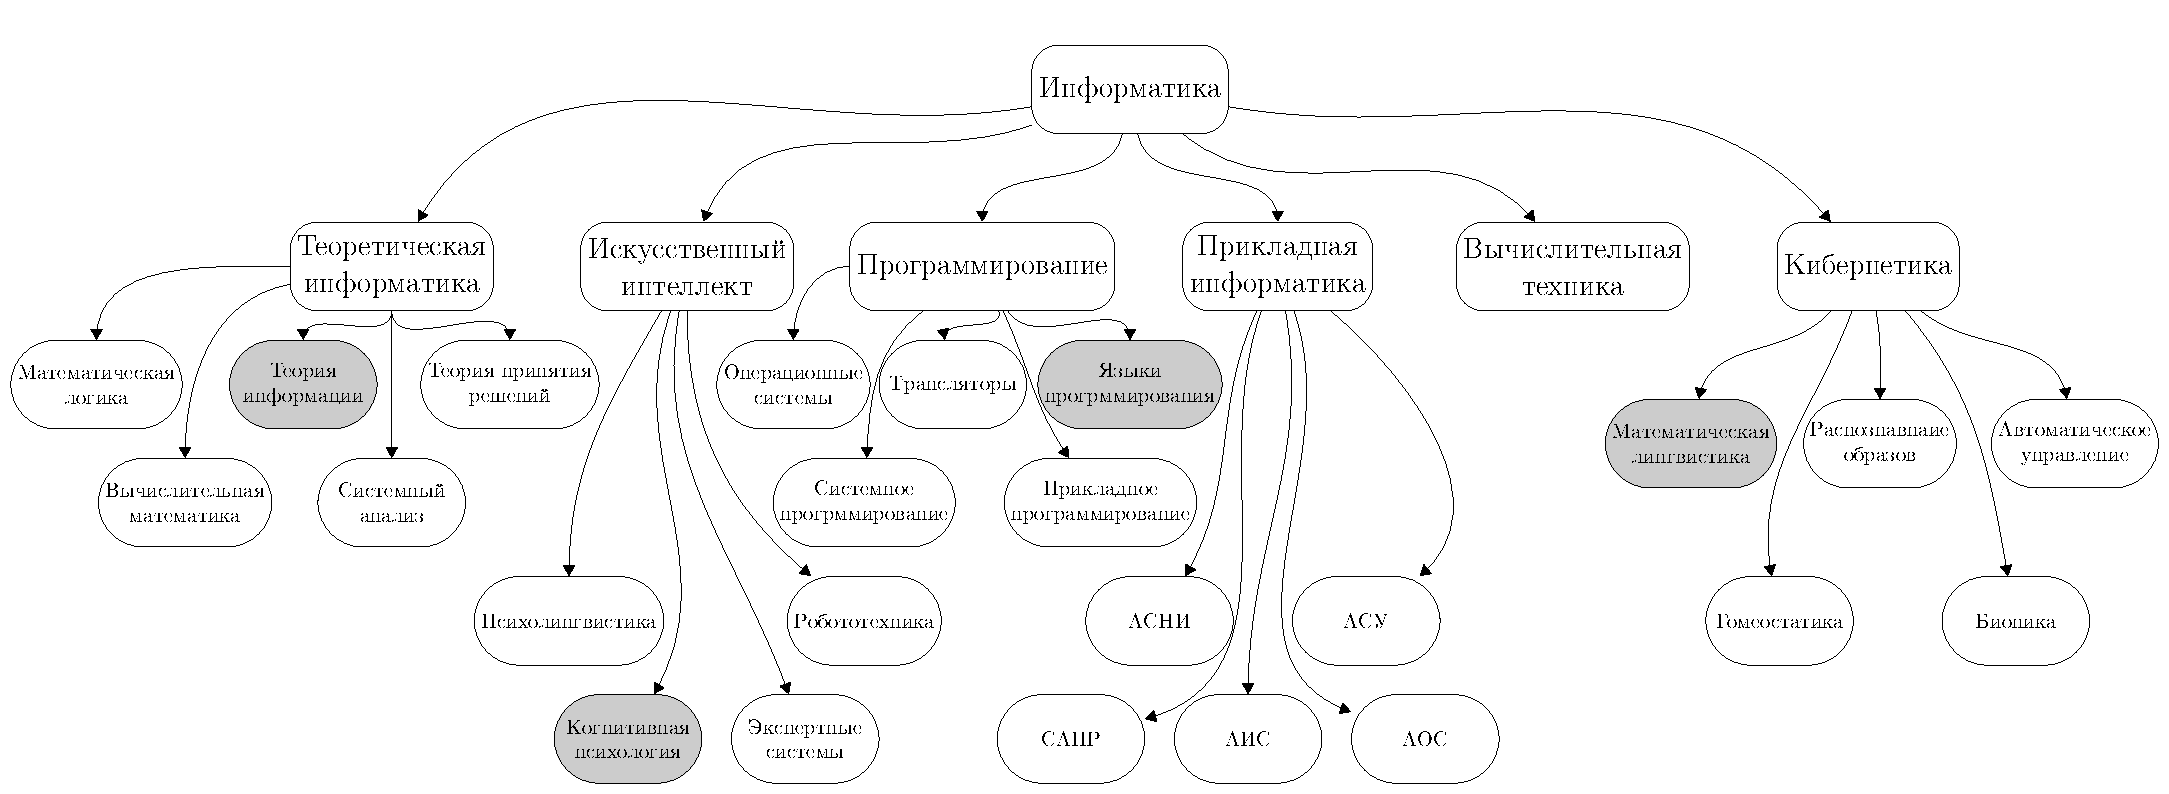
\includegraphics[width=\linewidth]{./tbi-textbook/inform}
		\caption{Фрагмент структуры дисциплины Информатика}
	\end{figure}
	
	
	\chapter{Теория информации}
	
	\section{Информация по Харлти и Шеннону}
	See also http://pmpu.ru/vf4/shannon
http://saitviktor.ru/source1/Glava2.htm
	Один из первых вопросов, которым задаются при работе с информацией любого рода "--- это вопрос о ее количестве. Как было сказано во введении, во всех случаях, когда говорится об информации мы будем указывать конкретную знаковую систему, которая является носителем информации. Иными словами, мы будем далее задаваться вопросом какое количество информации содержится в сообщении, записанном с использованием той или иной знаковой системы.
	
	Пусть у нас есть алфавит $A_{01}$, состоящий из двух символов 0 и 1. Сколько потребуется символов для обозначения $N$ различных сообщений? Ральф Хартли предложил считать этот вопрос эквивалентным вопросу <<Сколько информации содержится в сообщении длиной $N$>>. Таким образом, мы получаем следующую формулу количества информация по Хартли:
	\begin{equation}
		I = \log_2N.
	\end{equation}
	Информация по Шеннону:
	\begin{equation}
		I = -\sum_{i=0}^{i=N} p_i\log_2p_i.
	\end{equation}
	\subsection{Задачи для семинарских занятий}
		Здесь и далее значком $\unrhd$ обозначены задачи решение которых рекомендуется оформить в виде программной реализации.
		\begin{enumerate}
			\item Вам известно, что Вася бросил кубик. Вася послал сообщение: <<Кубик упал на четную грань>>. Сколько информации в сообщении?
			\item Вам известно, что Вася бросил кубик. Вася послал сообщение: <<Кубик упал на грань 5>>. Сколько информации в сообщении?
			\item Маша загадала число $x$ от 1 до 256. Сколько информации содержится в сообщении: 
				\begin{enumerate}
					\item $x < 9$;
					\item $x > 224$;
					\item $x > 97$;
					\item $x < 129$?
				\end{enumerate}
			\item Вам известно, что поезд придет завтра где-то между 10.00 и 21.00. Вася послал сообщение <<Поезд придет между 12.00 и 14.00>>. Сколько информации в сообщении.
			\item Маша загадала целое число $x$ от 1 до 256. Вася задал вопросы Маше: <<$x$ больше 100?>>, <<$x$ больше 150?>> и т.\,д. Какие вопросы должен задавать Вася, чтобы быстрее отгадать число $x$? Сколько таких вопросов он должен задать?
			\item $\unrhd$ Алфавит содержит 4 буквы,~используемые с вероятностями $p_1$, $p_2$, $p_3$ и $p_4$. Сообщение состоит из одного символа. Вычислить количество информации в сообщении по формуле Шеннона, если
				\begin{enumerate}
					\item $p_1=0,2, p_2=0,3, p_3=0,4, p_4=0,1$;
					\item $p_1=p_2=p_3=p_4=0,25$;
					\item $p_1=p_2=p_3=0,01, p_4=0,97$.
				\end{enumerate}
			\item $\unrhd$ Проводится опыт с двумя исходами, вероятности которых $p_1$ и $p_2$. Построить график зависимости энтропии $H$ опыта от вероятности одного из исходов $p_1$. Когда энтропия $H$ максимальна?
			\item $\unrhd$ Задано сообщение из $N$ символов на алфавита из 5 букв: $a,b,c,d,e$. Определить частоту (вероятность) использования каждого символа и по формуле Шеннона вычислить информацию $I_1$, приходящуюся на один символ, и общее количество информации в сообщении. При каких значениях частот символов информация максимальна?
			\item Разрешение монитора $1920\times 1080$, число цветов "--- 32. Какой объем видеопамяти нужен для хранения 4 страниц изображения.
			\item Какой объем имеет аудиофайл, время звучания которого 4 минуты при частоте дискретизации 44,1 кГц и разрешении 16 бит?
		\end{enumerate}
	\section{Информация по Колмогорову}
	\section{Рекурсия и количество информации}
	
	
	\chapter{Представление данных}
	В общем о данных
	
	\section{Графы}
	
	\section{Сети}
	
	\section{Операции над данными}
	
	\chapter{Представление знаний}
	В общем о знаниях
	
	\section{Теория автоматов}
	\section{Формальные грамматики}
	\section{Формальные языки и системы}
	\section{Теорема Гёделя}
	
	\chapter{Теория алгоритмов}
	
	\section{Простейшие алгоритмы}
	\section{Основы теории сложности}
	\section{Алгоритмы на строках}
	\section{Алгоритмы на графах}
	\section{Алгоритмы в экономике}
	
	
	\chapter*{Заключение}
	\addcontentsline{toc}{chapter}{Заключение}
	Немного о целях курса
	\printbibliography
\end{document}